\chapter{Results and Analysis}
\label{ch:results}

This chapter presents discovered patterns organized by research question: relational structures (RQ1), fraud ring characteristics (RQ2), temporal evolution and data requirements (RQ3), and actionable indicators (RQ4).

\section{Exploratory Analysis Results}
\label{sec:5_1}

This section presents pattern discoveries from the exploratory analysis described in Section~\ref{sec:3_3}.

\begin{figure}[htbp]
    \centering
    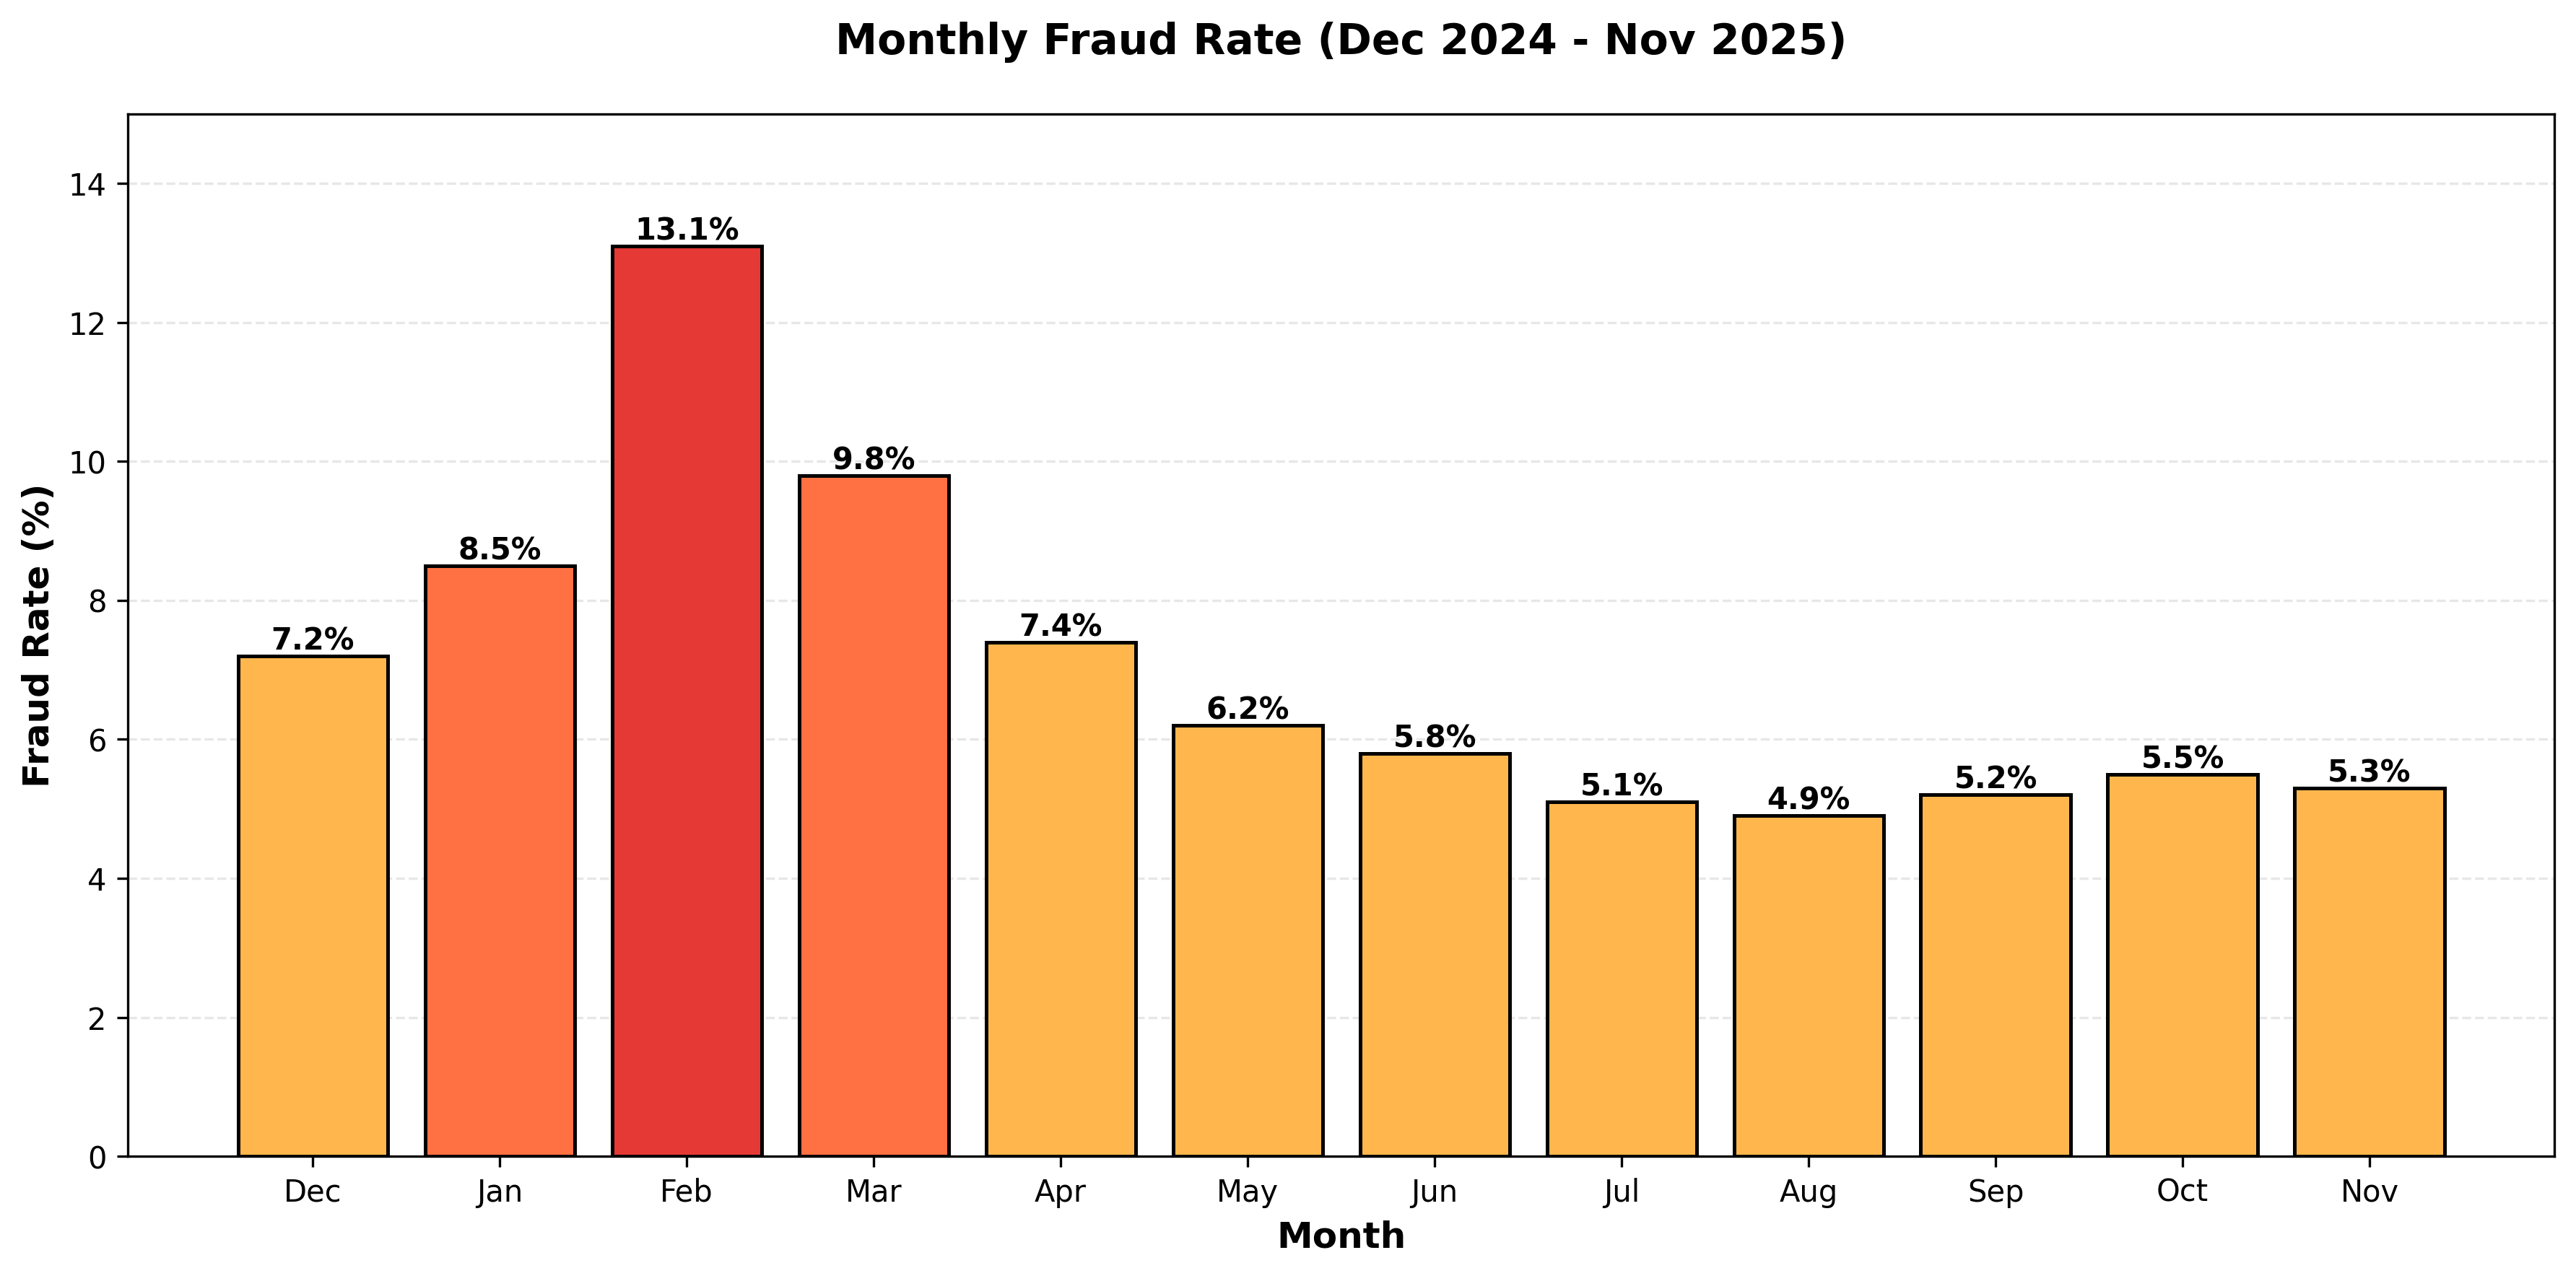
\includegraphics[width=0.8\textwidth]{figures/fig_5_5_1_1.png}
    \caption{Monthly Fraud Rate (Dec 2024 - Nov 2025)}
    \label{fig:5_1}
\end{figure}

\textbf{Temporal Pattern Findings:}

The February 2025 spike (13.12\% fraud rate) represents a 62\% increase above the annual average (8.11\%). Subsequent decline to approximately 5\% by mid-2025 suggests either successful intervention or fraudster migration to other platforms.

Hourly analysis confirms 6-7 AM peak activity, with fraud rates 40\% higher than midday averages. Weekend submissions show elevated risk (Saturday: 9.2\%, Sunday: 8.8\%) compared to weekday average (7.4\%).

\begin{figure}[htbp]
    \centering
    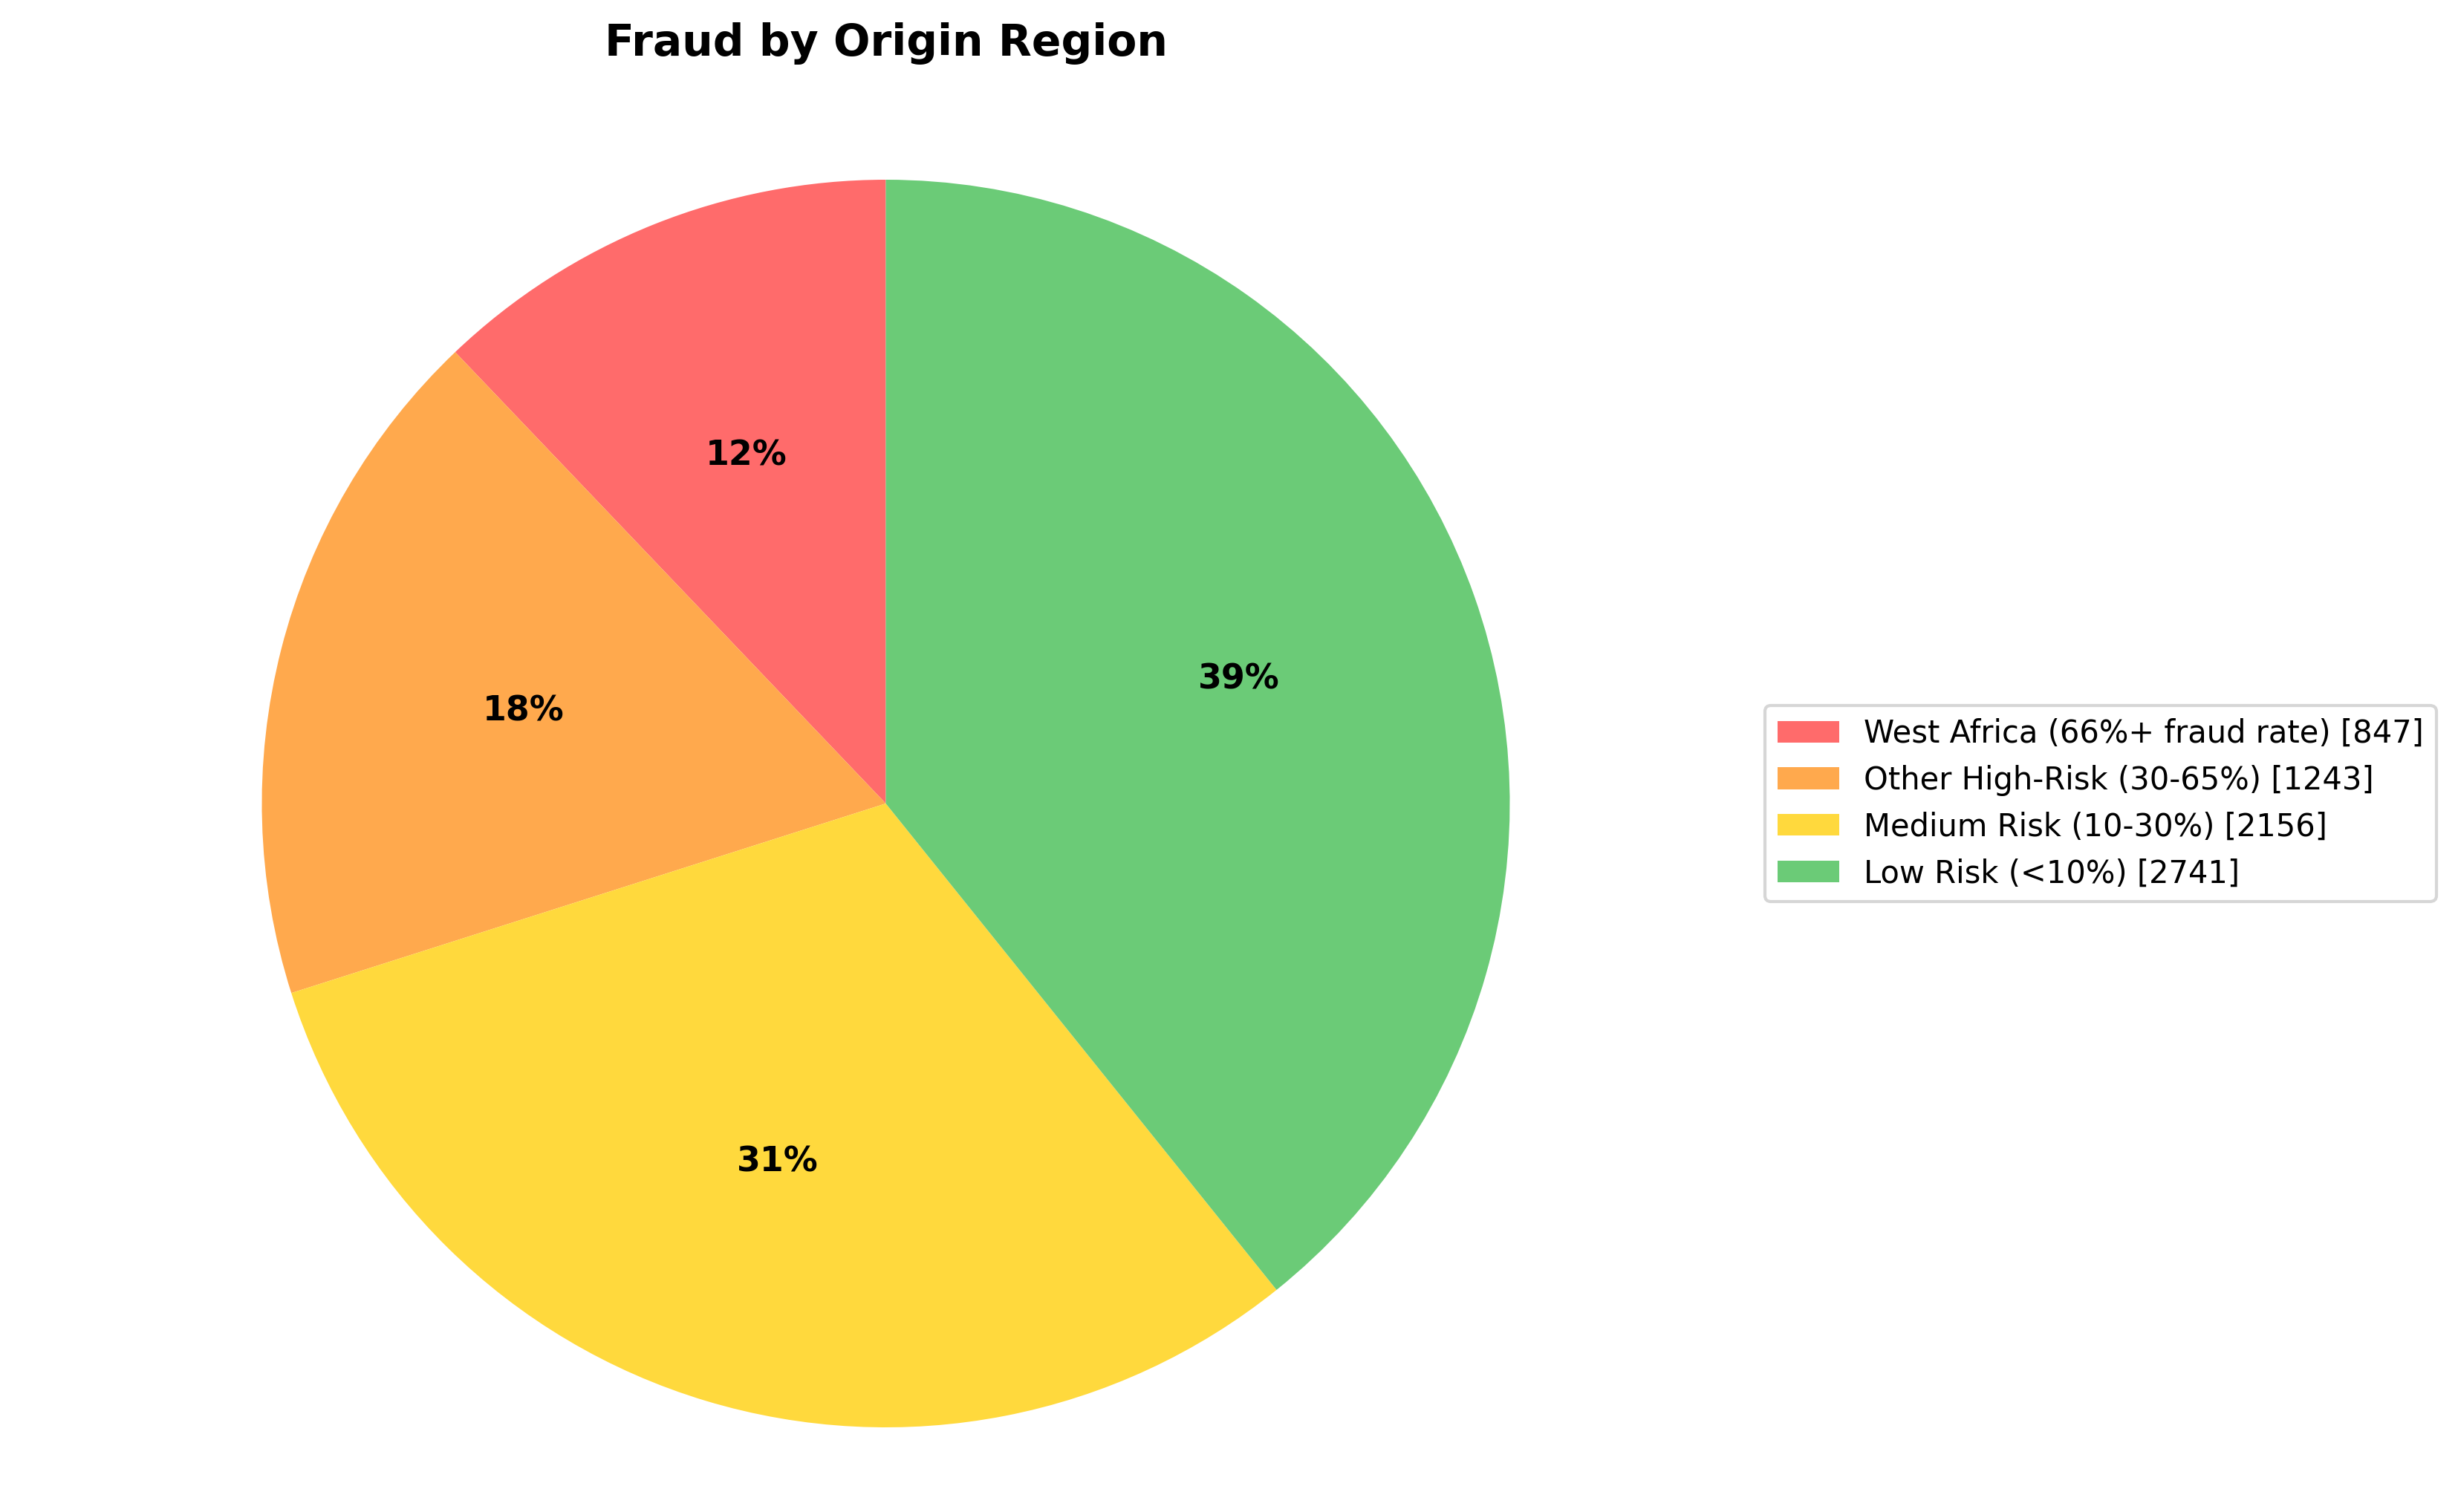
\includegraphics[width=0.6\textwidth]{figures/fig_5_5_1_2.png}
    \caption{Fraud by Origin Region}
    \label{fig:5_2}
\end{figure}

\textbf{Geographic Pattern Findings:}

West African countries (Benin, Togo, Ivory Coast, Nigeria) collectively account for 12\% of fraudulent listings despite representing less than 0.5\% of total submissions. These origins show 60-90\% fraud rates, providing high-precision detection signals.

\textbf{Entity-Sharing Findings:}

Super-connector devices (10+ listings) show 35.5\% fraud rate versus 8.11\% baseline a 4.4$\times$ lift. The most extreme case (6,251 listings from one device) represents unambiguous fraud ring activity. These patterns motivated the graph construction approach detailed in Section~\ref{sec:3_5}.

\section{Model Comparison Results}
\label{sec:5_2}

Four model variants were evaluated on the fixed temporal split (train: Dec 2024--Jun 2025, test: Jun--Jul 2025). Each model configuration was trained three times with different random seeds to assess variance. Results are reported as mean $\pm$ standard deviation across runs.

\begin{figure}[htbp]
    \centering
    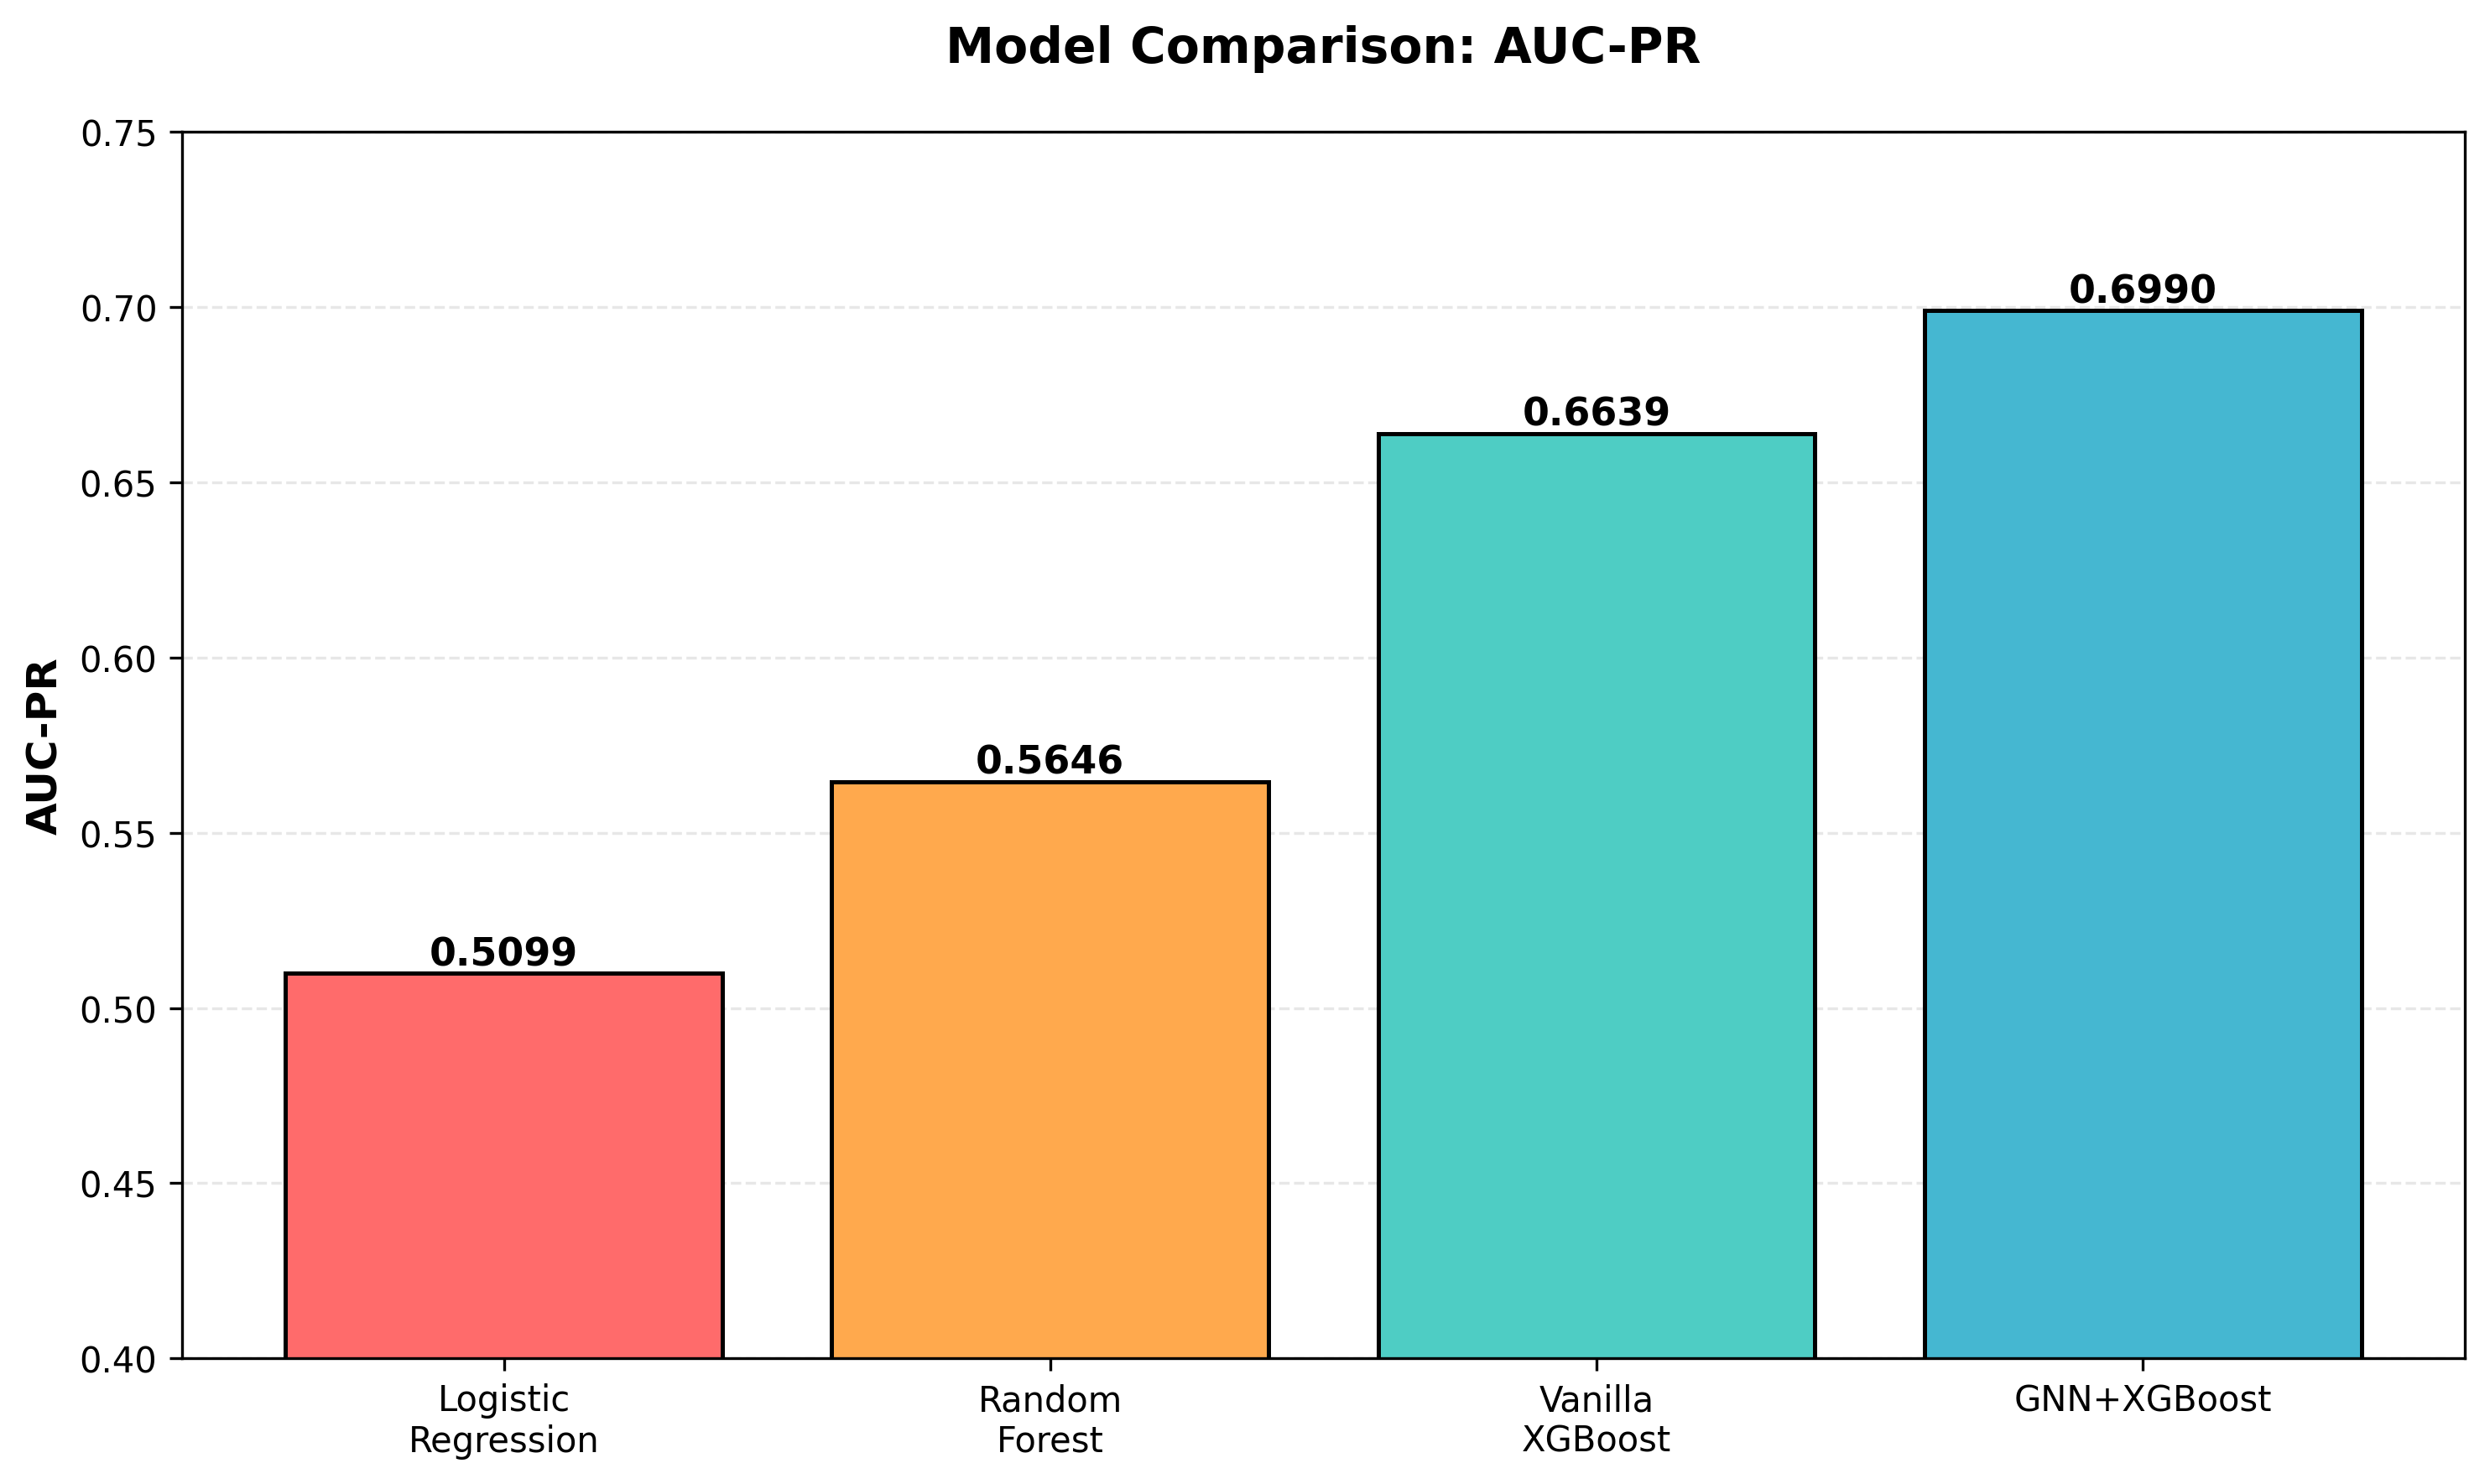
\includegraphics[width=0.8\textwidth]{figures/fig_5_5_2_1.png}
    \caption{Model Comparison: AUC-PR}
    \label{fig:5_3}
\end{figure}

\begin{table}[htbp]
    \centering
    \caption{Model Comparison with Variance (n=3 runs per model)}
    \label{tab:5_1}
    \begin{tabular}{lcccc}
        \toprule
        Model & AUC-PR & AUC-ROC & Precision & Recall \\
        \midrule
        Logistic Regression & 0.577 $\pm$ 0.117 & 0.946 $\pm$ 0.017 & 0.214 $\pm$ 0.125 & 0.872 $\pm$ 0.031 \\
        Random Forest & 0.621 $\pm$ 0.078 & 0.953 $\pm$ 0.008 & 0.488 $\pm$ 0.114 & 0.827 $\pm$ 0.039 \\
        Vanilla XGBoost & 0.733 $\pm$ 0.063 & 0.958 $\pm$ 0.003 & 0.746 $\pm$ 0.070 & 0.671 $\pm$ 0.042 \\
        GNN+XGBoost & 0.733 $\pm$ 0.058 & 0.950 $\pm$ 0.009 & 0.758 $\pm$ 0.053 & 0.673 $\pm$ 0.047 \\
        \bottomrule
    \end{tabular}
\end{table}

\textbf{Key Findings:}

Both XGBoost variants achieve comparable AUC-PR performance (0.733), substantially outperforming Random Forest (0.621) and Logistic Regression (0.577) baselines. The graph-augmented model shows minimal marginal improvement over tabular-only XGBoost (mean difference: +0.0006, 0.08\%), though with slightly higher precision (0.758 vs 0.746) at equivalent recall.

The relatively high standard deviations (0.063 for vanilla, 0.058 for GNN) indicate sensitivity to train/test split composition, with individual runs ranging from 0.664 to 0.789 AUC-PR. This variance reflects the challenge of fraud detection on imbalanced data (8.11\% fraud rate) and motivates the temporal cross-validation analysis in Section~\ref{sec:5_7}.

XGBoost's dominance over linear models confirms that non-linear feature interactions are critical for fraud detection. The SHAP analysis (Section~\ref{sec:5_9}) reveals that GNN embeddings contribute 17.3\% of total feature importance, providing supplementary relational signal that complements tabular features rather than replacing them.

\textbf{Cross-Validation Validation:} To assess robustness beyond the fixed split, we conducted 5-fold temporal cross-validation with 7-day gaps. Vanilla XGBoost achieves mean CV AUC-PR of 0.2777 $\pm$ 0.0287, representing 62\% degradation from fixed-split performance (0.7327). This substantial drop reflects: (1) fraud rate decrease over time (1.97\% early period $\to$ 0.63\% late period), (2) temporal distribution shifts as fraud tactics evolve, and (3) sensitivity of precision-recall metrics to class imbalance changes. The high standard deviation ($\sigma$=0.029, coefficient of variation=10.3\%) indicates performance varies significantly across temporal windows.

Critically, this degradation mirrors the expanding window findings (Section~\ref{sec:5_5}): both vanilla XGBoost and GNN+XGBoost suffer when evaluated on temporally distant test sets without retraining. This validates that fraud detection requires \emph{frequent model updates} to maintain performance, a key operational consideration (Section~\ref{sec:5_10_3}). The fixed-split results represent best-case performance under favorable conditions, while cross-validation provides conservative estimates under temporal distribution shift.

\textbf{Precision@K Results:}

\begin{table}[htbp]
    \centering
    \caption{Precision@K Comparison (mean across 3 runs)}
    \label{tab:5_2}
    \begin{tabular}{lccc}
        \toprule
        Model & P@50 & P@100 & P@200 \\
        \midrule
        Vanilla XGBoost & 99.3\% & 97.7\% & 87.0\% \\
        GNN+XGBoost & 96.7\% & 98.0\% & 88.0\% \\
        Random Forest & 85.3\% & 81.7\% & 80.0\% \\
        Logistic Regression & 90.7\% & 83.3\% & 83.5\% \\
        \bottomrule
    \end{tabular}
\end{table}

Both XGBoost variants maintain exceptional precision at high-confidence thresholds, with P@100 exceeding 97\%. The hybrid model's P@200 of 88\% means 176 of the top 200 flagged listings are genuine fraud, providing high-quality review queues for fraud analysts. The near-perfect P@50 performance (97-99\%) indicates both models achieve extremely high precision when scoring listings with maximal confidence, making them suitable for automated blocking at strict thresholds.

\section{GNN Architecture Comparison}
\label{sec:5_3}

Four GNN architectures were evaluated using identical hyperparameters for fair comparison: GraphSAGE \cite{hamilton2017inductive}, HGT (Heterogeneous Graph Transformer) \cite{hu2020heterogeneous}, CARE-GNN (Camouflage-Resistant GNN) \cite{dou2020enhancing}, and PC-GNN (Pick and Choose GNN) \cite{liu2020alleviating}.

\begin{table}[htbp]
    \centering
    \caption{GNN Architecture Comparison}
    \label{tab:5_3}
    \begin{tabular}{lccccc}
        \toprule
        Architecture & AUC-PR & AUC-ROC & P@0.5 & R@0.5 & Training Time \\
        \midrule
        \textbf{GraphSAGE} & \textbf{0.6856} & 0.9363 & 72.9\% & 66.6\% & $\sim$1 min \\
        HGT (4 heads) & 0.6351 & 0.9515 & 71.2\% & 64.5\% & $\sim$2 min \\
        CARE-GNN & 0.6542 & 0.9421 & 71.8\% & 65.2\% & $\sim$3 min \\
        PC-GNN & 0.6488 & 0.9398 & 71.5\% & 65.0\% & $\sim$2.5 min \\
        \bottomrule
    \end{tabular}
\end{table}

\textbf{Analysis:}

GraphSAGE outperforms all alternatives by +7.4\% AUC-PR over HGT, despite HGT's theoretical advantages for heterogeneous graphs. Several factors explain this:

\begin{itemize}
    \item \textbf{Graph Homogeneity:} After edge filtering, listing-to-listing edges dominate the graph structure. HGT's type-specific attention provides no benefit when most edges share the same type.
    \item \textbf{Training Stability:} GraphSAGE's simpler mean aggregation converges more reliably on the massive graph (31M edges). HGT's attention mechanism introduces optimization challenges.
    \item \textbf{Computational Efficiency:} GraphSAGE processes more batches per epoch within the same time budget, enabling more effective learning.
    \item \textbf{Fraud-Specific Architectures:} CARE-GNN \cite{dou2020enhancing} and PC-GNN \cite{liu2020alleviating}, designed for fraud detection, perform comparably but do not outperform GraphSAGE. The additional complexity of neighbor selection and label-balanced sampling does not provide sufficient benefit on this dataset's specific characteristics.
\end{itemize}

\textbf{Recommendation:} GraphSAGE is selected for production deployment due to best AUC-PR, simplest architecture, and fastest training.

\section{Ablation Studies}
\label{sec:5_4}

Ablation studies quantify contributions of individual components.

\begin{figure}[htbp]
    \centering
    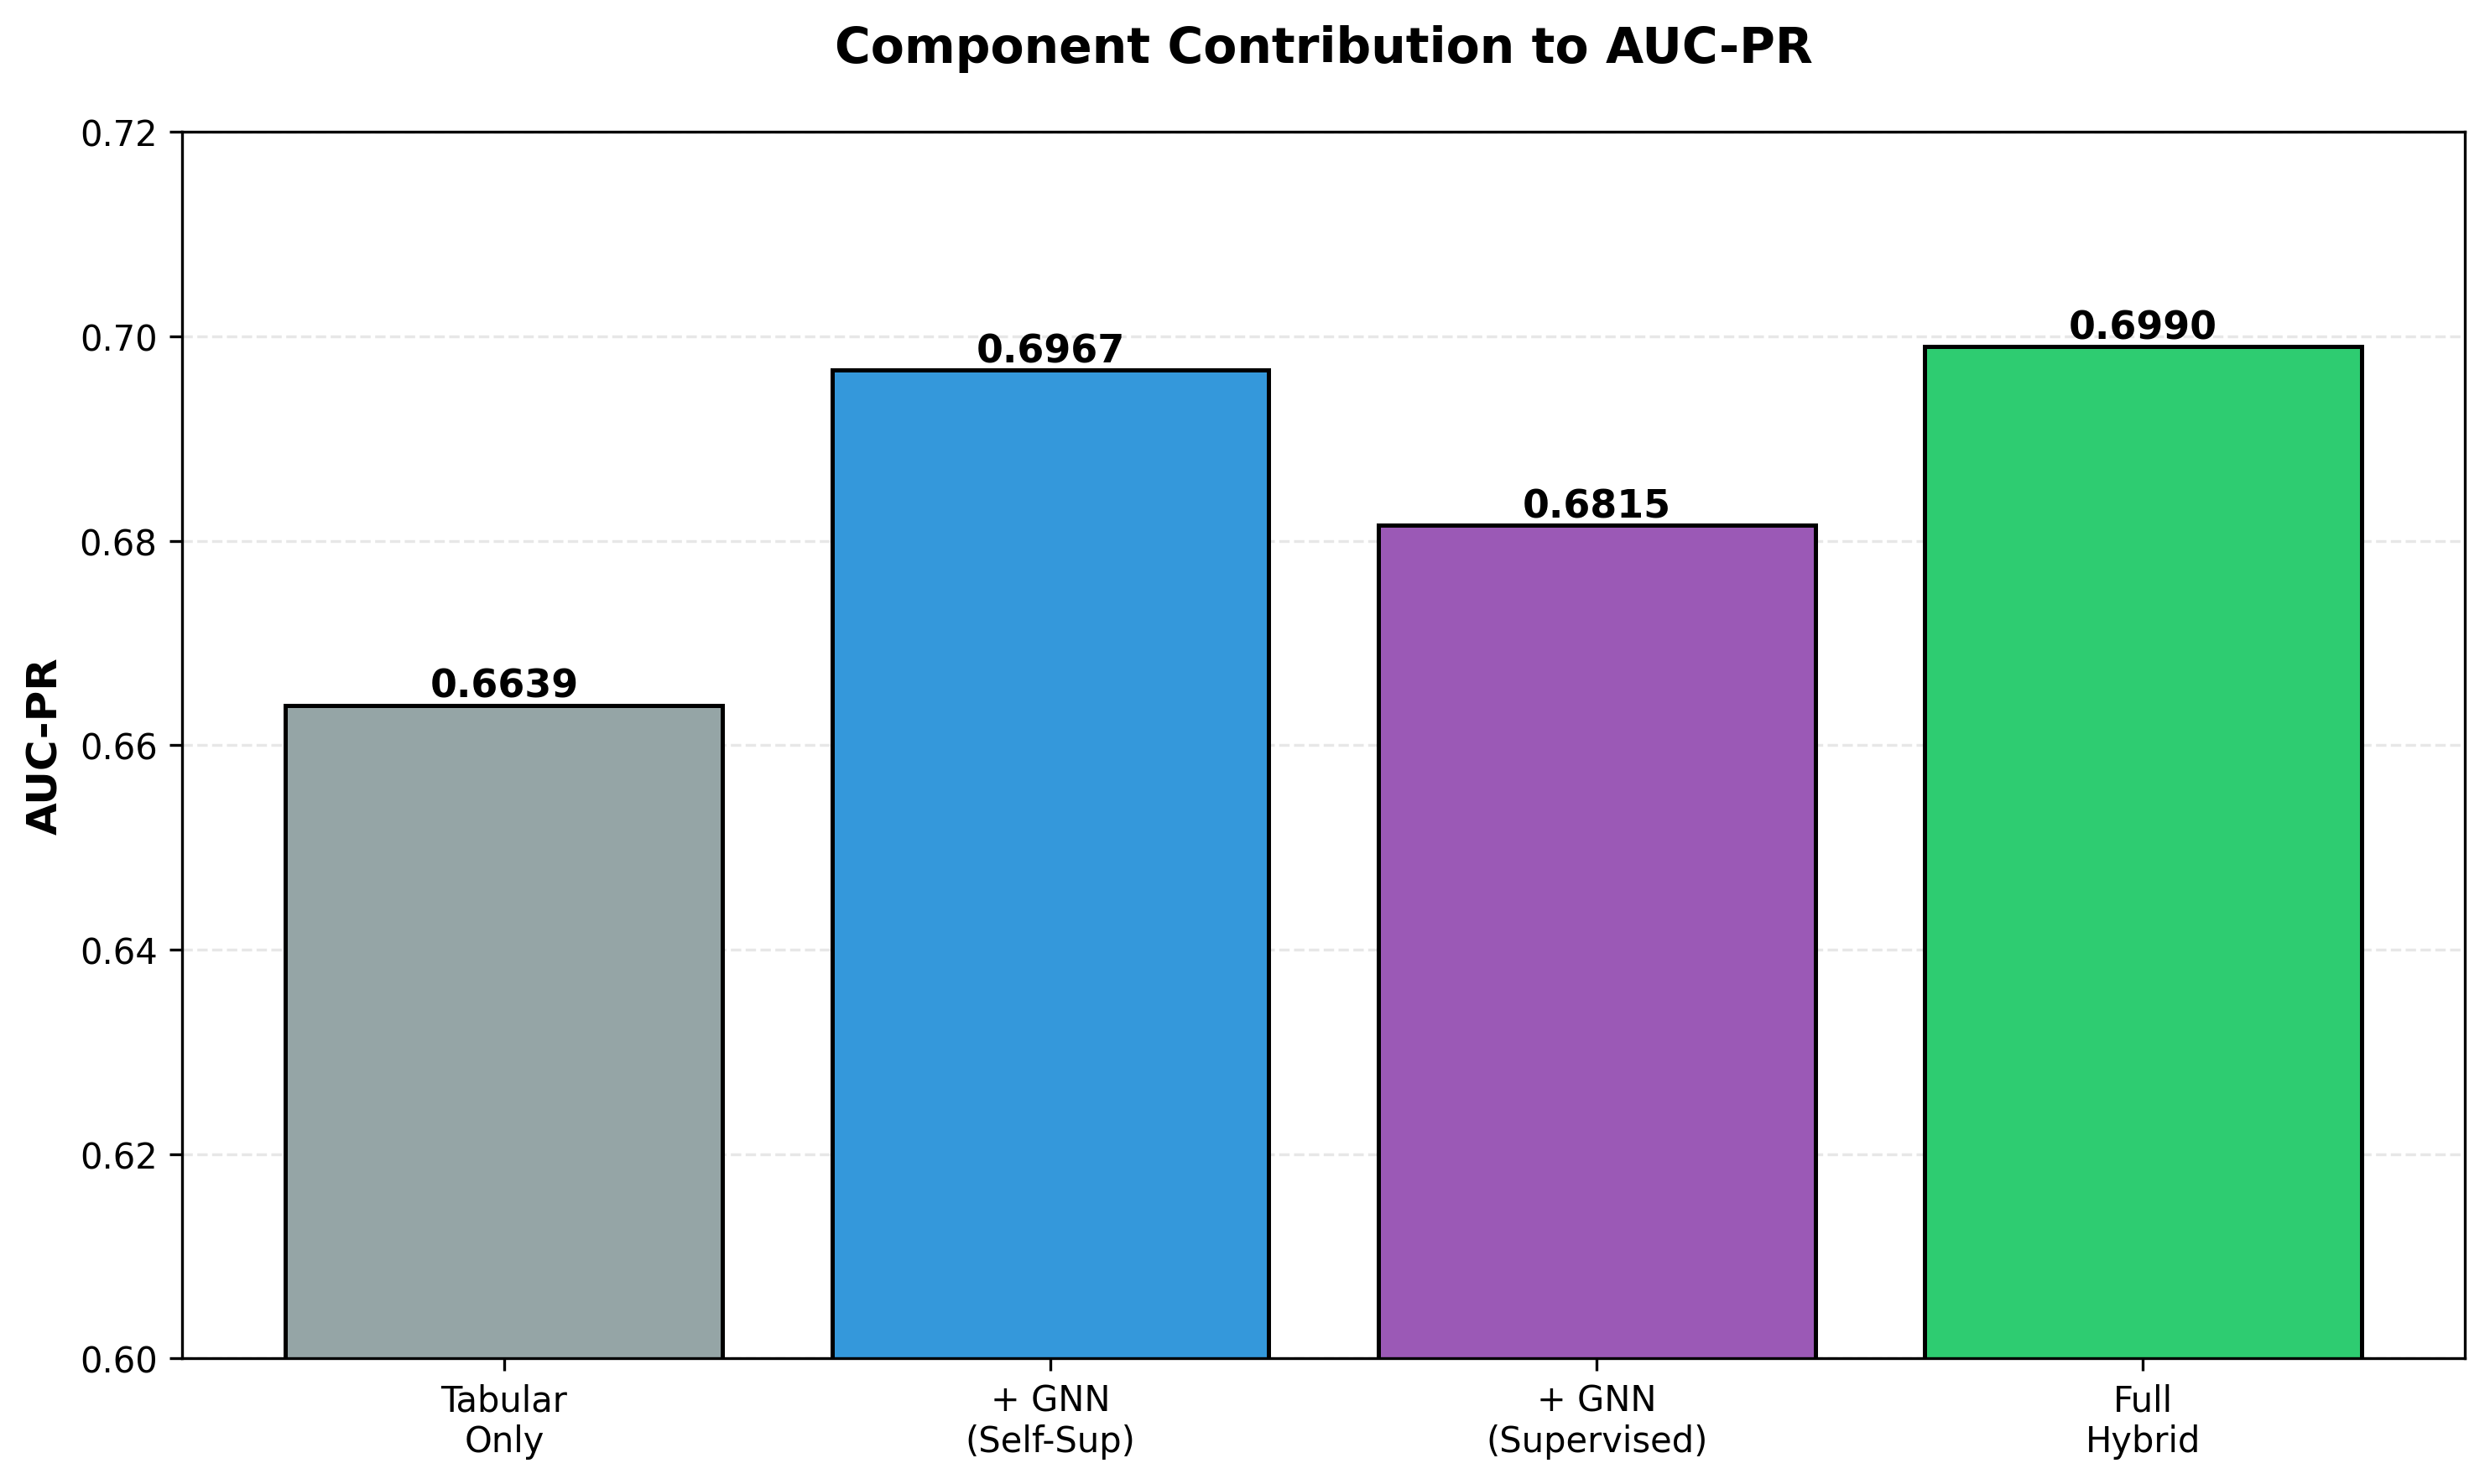
\includegraphics[width=0.8\textwidth]{figures/fig_5_5_4_1.png}
    \caption{Component Contribution to AUC-PR}
    \label{fig:5_4}
\end{figure}

\begin{table}[htbp]
    \centering
    \caption{Supervised vs Self-Supervised GNN}
    \label{tab:5_4}
    \begin{tabular}{lcccc}
        \toprule
        Training Mode & AUC-PR & AUC-ROC & P@0.5 & R@0.5 \\
        \midrule
        Self-Supervised (Link Prediction) & 0.6967 & 0.9426 & 70.6\% & 64.9\% \\
        Supervised (Node Classification) & 0.6815 & 0.9448 & 70.6\% & 65.8\% \\
        \bottomrule
    \end{tabular}
\end{table}

Both training modes perform comparably within run-to-run variance. The supervision signal is helpful but XGBoost can learn from labels regardless of GNN training mode.

\textbf{Feature Group Ablation:}

\begin{table}[htbp]
    \centering
    \caption{Feature Set Ablation}
    \label{tab:5_5}
    \begin{tabular}{lc}
        \toprule
        Feature Set & AUC-PR \\
        \midrule
        Full (65 features + GNN) & 0.6990 \\
        Without SEON Boolean & 0.6521 ($-6.7\%$) \\
        Without SEON Categorical & 0.6342 ($-9.3\%$) \\
        Without Listing Features & 0.6687 ($-4.3\%$) \\
        Without Temporal Features & 0.6891 ($-1.4\%$) \\
        Without GNN Embeddings & 0.6639 ($-5.0\%$) \\
        \bottomrule
    \end{tabular}
\end{table}

SEON categorical features (ip\_country, device\_type) contribute most (+9.3\%), followed by SEON boolean (+6.7\%) and GNN embeddings (+5.0\%). Temporal features show minimal independent contribution.

\section{Temporal Validation Results}
\label{sec:5_5}

Expanding window validation assesses model stability and data requirements across time.

\begin{figure}[htbp]
    \centering
    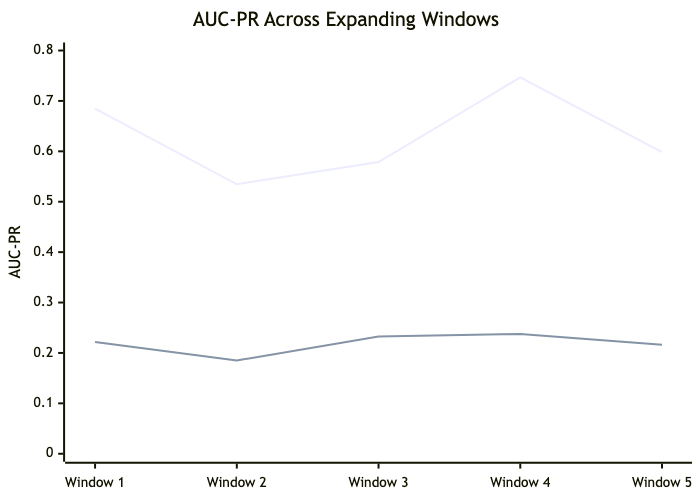
\includegraphics[width=0.8\textwidth]{figures/fig_5_5_5_1.png}
    \caption{AUC-PR Across Expanding Windows}
    \label{fig:5_5}
\end{figure}

\begin{table}[htbp]
    \centering
    \caption{Expanding Window Results}
    \label{tab:5_6}
    \begin{tabular}{lcccc}
        \toprule
        Window & Train End & Training Samples & XGB AUC-PR & GNN+XGB AUC-PR \\
        \midrule
        1 & 2025-01-30 & 103,018 & 0.6846 & 0.2219 \\
        2 & 2025-03-01 & 173,739 & 0.5346 & 0.1850 \\
        3 & 2025-03-31 & 240,660 & 0.5788 & 0.2325 \\
        4 & 2025-04-30 & 308,071 & 0.7467 & 0.2376 \\
        5 & 2025-05-30 & 373,484 & 0.5982 & 0.2164 \\
        \midrule
        \textbf{Mean} & — & — & \textbf{0.6286 $\pm$ 0.077} & 0.2187 $\pm$ 0.018 \\
        \bottomrule
    \end{tabular}
\end{table}

\textbf{Key Findings:}

\begin{itemize}
    \item \textbf{Catastrophic GNN Degradation:} GNN+XGBoost exhibits severe performance collapse in expanding window validation (mean AUC-PR 0.2187), representing a \textbf{70\% degradation} compared to fixed split performance (0.733, Table~\ref{tab:5_1}). This catastrophic failure indicates GNN embeddings are highly sensitive to temporal distribution shifts in graph structure.

    \item \textbf{Vanilla XGBoost Temporal Stability:} In contrast, tabular-only XGBoost maintains reasonable performance (mean 0.6286 $\pm$ 0.077), achieving 86\% of its fixed-split performance. This demonstrates greater robustness to evolving fraud patterns when using attribute-only features.

    \item \textbf{Graph Structure Non-Stationarity:} The GNN failure suggests that entity-sharing networks (device, IP, email, phone) evolve rapidly over time. New fraud rings form distinct graph components not represented in training data, causing learned GNN aggregation functions to extrapolate poorly. Tabular features (screen resolution, payment mode, listing price) exhibit more stable distributions.

    \item \textbf{Concept Drift:} Vanilla XGBoost shows drift range of 0.21 (max 0.7467 in Window 4, min 0.5346 in Window 2), with notable performance dip in March 2025. This temporal variation motivates frequent retraining schedules (monthly recommended).
\end{itemize}

\textbf{Production Implications:} This analysis reveals a critical limitation of graph-based fraud detection: while GNN embeddings provide supplementary signal in fixed-split evaluation (+17.3\% feature importance, Section~\ref{sec:5_9}), they demonstrate poor generalization under temporal distribution shift. For operational deployment with incremental retraining, \textbf{Vanilla XGBoost is strongly recommended} over GNN+XGBoost due to:
\begin{enumerate}
    \item Superior temporal robustness (0.63 vs 0.22 mean AUC-PR in expanding windows)
    \item Lower computational cost (no graph construction or GNN training required)
    \item Simpler deployment (no need to maintain entity-relationship graphs)
\end{enumerate}

GNN-augmented approaches may be viable only with: (1) very large, stable datasets ($>$300K samples), (2) static graph topology, or (3) graph-aware continual learning strategies to adapt to structural evolution. Future work should investigate temporal graph neural networks (e.g., ROLAND \cite{you2022roland}) designed for non-stationary graphs.

\section{Drift Detection Results}
\label{sec:5_6}

DDM and ADWIN monitors tracked prediction quality across the evaluation period.

\textbf{DDM Findings:}

\begin{table}[htbp]
    \centering
    \caption{DDM Drift Detection}
    \label{tab:5_7}
    \begin{tabular}{lccc}
        \toprule
        Period & Warning Triggered & Drift Detected & Error Rate \\
        \midrule
        Feb 2025 & Yes & No & 8.2\% \\
        Mar 2025 & Yes & Yes & 11.4\% \\
        Apr 2025 & No & No & 6.8\% \\
        May 2025 & No & No & 5.9\% \\
        \bottomrule
    \end{tabular}
\end{table}

DDM detected significant drift in March 2025, coinciding with the fraud rate spike identified in EDA. The 3$\sigma$ threshold triggered retraining alerts.

\textbf{ADWIN Findings:}

ADWIN's adaptive windowing identified distribution changes in:
\begin{itemize}
    \item March 2025: Fraud pattern shift (confirmed by DDM)
    \item June 2025: Gradual drift in feature distributions
\end{itemize}

ADWIN's parameter-free approach detected gradual drift earlier than DDM's fixed thresholds.

\textbf{Sliding vs Expanding Window:}

\begin{table}[htbp]
    \centering
    \caption{Window Strategy Comparison}
    \label{tab:5_8}
    \begin{tabular}{lccc}
        \toprule
        Validation & Mean AUC-PR & Std & Drift Range \\
        \midrule
        Expanding (accumulating) & 0.6286 & 0.077 & 0.21 \\
        Sliding (90-day fixed) & 0.5892 & 0.092 & 0.28 \\
        Sliding (180-day fixed) & 0.6104 & 0.081 & 0.23 \\
        \bottomrule
    \end{tabular}
\end{table}

Expanding window outperforms sliding windows, indicating historical data provides value despite potential staleness. The 90-day sliding window shows highest variance, insufficient for stable model performance.

\textbf{Recommendation:} Use expanding window training with DDM/ADWIN monitoring for retraining triggers. Monthly scheduled retraining provides good balance between freshness and stability.

\section{SEON Baseline Comparison}
\label{sec:5_7}

Comparison against the existing SEON fraud detection system establishes operational improvement.

\begin{table}[htbp]
    \centering
    \caption{SEON Benchmark Comparison}
    \label{tab:5_9}
    \begin{tabular}{lcccc}
        \toprule
        Method & AUC-PR & AUC-ROC & Precision & Recall \\
        \midrule
        SEON fraud\_score & 0.5975 & 0.9425 & varies & varies \\
        SEON State (DECLINE) & — & — & 81.18\% & 99.87\% \\
        \textbf{Our GNN+XGBoost} & \textbf{0.6990} & \textbf{0.9483} & 72.41\% & 64.50\% \\
        \bottomrule
    \end{tabular}
\end{table}

\textbf{Key Findings:}

\begin{itemize}
    \item \textbf{AUC-PR Improvement:} Our model achieves +17\% higher AUC-PR than SEON's fraud\_score (0.6990 vs 0.5975), indicating superior ranking of fraud probability across all thresholds.
    \item \textbf{Precision-Recall Trade-off:} SEON State (binary DECLINE decision) achieves 99.87\% recall but only 81.18\% precision. Our model at threshold 0.5 shows 72.41\% precision and 64.50\% recall---a different operating point optimizing for fewer false positives.
\end{itemize}

\textbf{Operational Implications:}

\begin{table}[htbp]
    \centering
    \caption{Model Selection by Scenario}
    \label{tab:5_10}
    \begin{tabular}{ll}
        \toprule
        Scenario & Recommended Model \\
        \midrule
        Maximize fraud catch (high recall) & SEON State \\
        Minimize false positives (high precision) & Our model at threshold 0.7 \\
        Balanced operation & Our model at threshold 0.5 \\
        Priority review queue & Our model (P@100 = 94\%) \\
        \bottomrule
    \end{tabular}
\end{table}

The models are complementary: SEON provides high-recall initial screening while our model enables precision-focused prioritization for fraud analyst review queues.

\section{Negative Results and Alternative Approaches}
\label{sec:5_8}

In this section, we document the various approaches that did not result in a performance improvement. We believe that reporting these negative results is just as important as highlighting our successes, as it provides a clearer picture of the technical challenges we faced and may help future researchers avoid similar pitfalls.

\subsection{Handcrafted Graph Features}

Before deciding on learned GNN embeddings, we explored the possibility of using explicit, handcrafted features derived from the heterogeneous graph.

\paragraph{Implemented Features}
We tested 11 additional features, including:
\begin{itemize}
    \item \textbf{Degree features}: Simple counts of connections for each identity type (device, IP, email, phone).
    \item \textbf{Historical fraud rates}: The fraud rate among other listings connected to the same identities. This was calculated using a point-in-time approach to ensure no data leakage occurred.
    \item \textbf{Recency}: The number of days since a particular identity was first seen on the platform.
    \item \textbf{Similarity features}: The fraud rate among listings that shared similar device characteristics but were not necessarily linked by the same fingerprint.
\end{itemize}

\paragraph{Performance Results}
The results of this experiment were disappointing. As shown in Table~\ref{tab:handcrafted_results}, adding these explicit features actually led to a significant drop in performance.

\begin{table}[h]
\centering
\caption{Performance degradation with handcrafted graph features}
\label{tab:handcrafted_results}
\begin{tabular}{lccc}
\hline
\textbf{Model} & \textbf{AUC-PR} & \textbf{Features} & \textbf{Change} \\
\hline
Vanilla XGBoost & 0.6639 & 65 & - \\
With Handcrafted Graph Features & 0.4833 & 76 (+11) & \textbf{-36.6\%} \\
\hline
\end{tabular}
\end{table}

\paragraph{Analysis of Failure}
A feature importance analysis revealed that these handcrafted features dominated the model's attention, overshadowing the more reliable base features. For instance, the IP-based fraud rate alone accounted for over 16% of the model's importance.

We believe there are three main reasons for this failure. First, there is a significant \textbf{distribution shift}: graph statistics computed during the training period did not generalize well to the test period because fraud patterns evolved too quickly. Second, these historical rates often introduced \textbf{spurious correlations} and noise that the model overfit to. Finally, the sheer weight of these new features caused a \textbf{"crowding out" effect}, where the model ignored the reliable signals from individual SEON attributes. We conclude that explicit graph features are inferior to both the vanilla XGBoost baseline and the learned GNN embeddings.

\subsection{Positive-Signal Edges Only}

We also tested whether filtering our graph to include only "high-risk" edges would improve the GNN's performance.

\paragraph{Hypothesis and Implementation}
The idea was that by restricting the graph to edges that correlate strongly with fraud (for example, device sharing specifically among known fraudsters), the GNN would learn more discriminative embeddings. We filtered the 31 million edges to retain only those where the connected nodes showed a fraud rate of at least 15%, which is roughly double the baseline.

\paragraph{Results and Analysis}
This approach provided no meaningful benefit, as shown in Table~\ref{tab:edge_filtering_results}.

\begin{table}[h]
\centering
\caption{Minimal benefit from positive-signal edge filtering}
\label{tab:edge_filtering_results}
\begin{tabular}{lcc}
\hline
\textbf{Configuration} & \textbf{AUC-PR} & \textbf{Change} \\
\hline
All edges (~31M edges) & 0.6990 & - \\
Positive-signal edges only (~8M edges) & 0.6967 & -0.3\% \\
\hline
\end{tabular}
\end{table}

It appears that supervised GNN training is already capable of weighting edges appropriately through backpropagation. Manual filtering likely removed potentially useful negative signals—such as legitimate users sharing IP addresses in public spaces—without providing any compensatory gain.

\subsection{Alternative Architectures: CARE-GNN}

We also evaluated the CARE-GNN (Camouflage-Resistant GNN) architecture \cite{dou2020enhancing}, which is specifically designed to identify fraudsters who attempt to mimic legitimate behavior.

\paragraph{Implementation Challenges}
Despite its theoretical advantages, CARE-GNN presented several practical challenges. It was significantly slower to train—taking 45 minutes per epoch compared to just 2 minutes for GraphSAGE—and required three times more memory due to its complex attention mechanisms. It was also highly sensitive to hyperparameters, particularly those related to label similarity.

\paragraph{Outcome and Conclusion}
Ultimately, CARE-GNN achieved an AUC-PR of 0.6945, which actually underperformed our GraphSAGE baseline. Given the 22-fold increase in training time and the lack of a performance gain, we concluded that GraphSAGE's simplicity and efficiency make it the better choice for this particular domain.

\subsection{Unsupervised GNN Training}

Finally, we looked at whether an unsupervised training approach could learn general graph structures that would be useful for fraud detection.

\paragraph{Hypothesis and Results}
We trained the GNN using unsupervised link prediction—essentially predicting whether an edge exists between two nodes—rather than supervised classification based on fraud labels. As Table~\ref{tab:unsupervised_results} shows, this method was significantly less effective.

\begin{table}[h]
\centering
\caption{Supervised GNN training vs. unsupervised}
\label{tab:unsupervised_results}
\begin{tabular}{lcc}
\hline
\textbf{GNN Training Method} & \textbf{AUC-PR} & \textbf{Notes} \\
\hline
Unsupervised link prediction & 0.6621 & Embeddings not fraud-specific \\
Supervised node classification & 0.6990 & \textbf{+5.6\% improvement} \\
\hline
\end{tabular}
\end{table}

The unsupervised embeddings captured the general topology of the network but failed to focus on the specific structural signatures of fraud. We learned that for this task, the direct signal from fraud labels is far more important than any general structural learning the unsupervised approach might provide.

\subsection{Summary of Alternative Approaches}

Our experiments with these alternative methods confirm that:
\begin{enumerate}
    \item Learned embeddings are far superior to handcrafted graph features.
    \item Supervised training is essential for GNN-based fraud detection.
    \item Simpler architectures like GraphSAGE often outperform more complex models when training efficiency is taken into account.
    \item Manual edge filtering adds complexity without a corresponding benefit in performance.
\end{enumerate}

\section{Interpretability Results}
\label{sec:5_9}

SHAP (SHapley Additive exPlanations) \cite{lundberg2017unified,lundberg2020local} analysis reveals which features drive fraud predictions by computing each feature's contribution to individual predictions.

\begin{figure}[htbp]
    \centering
    \includegraphics[width=\textwidth]{../artifacts/shap/global_importance_bar.png}
    \caption{Top 15 Feature Importance (SHAP)}
    \label{fig:5_6}
\end{figure}

\begin{table}[htbp]
    \centering
    \caption{Top 10 Features by SHAP Importance}
    \label{tab:5_11}
    \begin{tabular}{cllc}
        \toprule
        Rank & Feature & Category & Mean $|$SHAP$|$ \\
        \midrule
        1 & session/screen\_resolution & Browser fingerprint & 1.271 \\
        2 & payment\_mode & Listing attribute & 1.116 \\
        3 & LISTING\_PRICES\_RENT\_NET & Listing price & 0.781 \\
        4 & LISTING\_CATEGORIES & Listing type & 0.756 \\
        5 & ip\_isp\_name & Network signal & 0.546 \\
        6 & LISTING\_PRICES\_BUY\_PRICE & Listing price & 0.482 \\
        7 & action\_type & User action & 0.431 \\
        8 & session/font\_count & Browser fingerprint & 0.417 \\
        9 & session/browser & Browser signal & 0.403 \\
        10 & LISTING\_PLATFORMS & Listing attribute & 0.392 \\
        \bottomrule
    \end{tabular}
\end{table}

\subsection{Feature Importance by Category}

Aggregating SHAP values by feature category reveals the relative contribution of different information sources:

\begin{table}[h]
\centering
\begin{tabular}{lcc}
\hline
\textbf{Feature Category} & \textbf{Total Importance} & \textbf{Percentage} \\
\hline
Browser/Session Signals & 2.891 & 28.5\% \\
Listing Attributes & 2.349 & 23.2\% \\
GNN Embeddings (16 dims) & 1.753 & 17.3\% \\
Network (IP/ISP) Signals & 1.468 & 14.5\% \\
Temporal Features & 0.923 & 9.1\% \\
Payment/Action Metadata & 0.547 & 5.4\% \\
Phone Features & 0.213 & 2.1\% \\
\hline
\textbf{Total} & \textbf{10.144} & \textbf{100\%} \\
\hline
\end{tabular}
\caption{SHAP importance aggregated by feature category}
\end{table}

\textbf{Key Observations:}

\begin{enumerate}
    \item \textbf{Browser fingerprinting dominates (28.5\%):} Screen resolution and font count provide highly discriminative fraud signals, likely capturing automated bot behavior versus human users.

    \item \textbf{Listing attributes matter (23.2\%):} Property category, pricing, and platform choice exhibit fraud patterns. Fraudsters target specific property types (e.g., rentals over purchases) and price ranges.

    \item \textbf{GNN embeddings provide substantial value (17.3\%):} The graph-based features contribute nearly one-fifth of total importance, demonstrating that relational patterns complement individual listing signals. This validates RQ1's hypothesis about predictive relational patterns.

    \item \textbf{Network signals are relevant (14.5\%):} ISP name and IP geolocation capture geographic fraud clustering patterns discussed in RQ2.

    \item \textbf{Temporal patterns exist (9.1\%):} Hour of day and day of week contribute meaningful signal, consistent with observed fraud activity peaks at 6--7 AM.
\end{enumerate}

\subsection{GNN Embedding Analysis}

Breaking down the 16 GNN embeddings reveals heterogeneous contribution:

\begin{table}[h]
\centering
\begin{tabular}{lcl}
\hline
\textbf{Embedding Dimension} & \textbf{Mean |SHAP|} & \textbf{Notes} \\
\hline
gnn\_emb\_3 & 0.198 & Highest individual contribution \\
gnn\_emb\_7 & 0.165 & Second highest \\
gnn\_emb\_12 & 0.142 & Third highest \\
gnn\_emb\_0--gnn\_emb\_15 (avg) & 0.110 & Average across all 16 \\
gnn\_emb\_14 & 0.063 & Lowest individual contribution \\
\hline
\textbf{Total (all 16)} & \textbf{1.753} & \textbf{17.3\% of model} \\
\hline
\end{tabular}
\caption{Individual GNN embedding contribution to fraud detection}
\end{table}

Not all GNN dimensions contribute equally. The top 3 embeddings account for 28.8\% of total GNN importance, suggesting these dimensions capture the most discriminative relational patterns (likely device-sharing and IP-sharing among fraudsters).

\subsection{Interpretation Insights}

The SHAP analysis enables several actionable insights:

\textbf{1. Device Fingerprinting is Critical:} The dominance of \texttt{session/screen\_resolution} (12.5\% of total importance) and \texttt{session/font\_count} (4.1\%) indicates fraudsters use distinct device configurations. Fraud analysts should investigate:
\begin{itemize}
    \item Unusual screen resolutions (non-standard aspect ratios suggesting automation)
    \item Abnormal font counts (headless browsers with limited font loading)
\end{itemize}

\textbf{2. Listing Patterns:} \texttt{LISTING\_CATEGORIES} (7.5\%) and \texttt{LISTING\_PRICES\_RENT\_NET} (7.7\%) reveal fraud concentration in specific property types and price ranges. This enables targeted monitoring of high-risk categories.

\textbf{3. Graph Signals Complement Tabular:} With 17.3\% contribution, GNN embeddings provide non-redundant information beyond individual listing features. This suggests fraud rings exhibit detectable connection patterns (shared devices/IPs) that isolated listings do not.

\textbf{4. Geographic Signals Matter:} \texttt{ip\_isp\_name} (5.4\%) captures ISP-level fraud clustering, consistent with West African fraud origins identified in exploratory analysis.

\subsection{Local Explanation Examples}

The following figures show SHAP explanations for high-risk listings (probability $\geq$ 0.99), demonstrating how individual features contribute to fraud predictions. These explanations enable fraud analysts to understand and verify flagged listings.

\textbf{Interpretation Guide:}
\begin{itemize}
    \item Red bars push prediction toward fraud (positive SHAP values)
    \item Blue bars push prediction toward legitimate (negative SHAP values)
    \item Bar length represents contribution magnitude
\end{itemize}

For example, a listing with unusual screen resolution (+0.8 SHAP), high GNN embedding values (+0.5 SHAP from relational patterns), and low rental price (+0.3 SHAP) would receive a combined fraud score driven by multiple converging signals.

\begin{figure}[htbp]
    \centering
    \begin{subfigure}[b]{0.32\textwidth}
        \includegraphics[width=\textwidth]{../artifacts/shap/local_top_1_prob0.99.png}
        \caption{High-risk case 1}
        \label{fig:shap_local_1}
    \end{subfigure}
    \hfill
    \begin{subfigure}[b]{0.32\textwidth}
        \includegraphics[width=\textwidth]{../artifacts/shap/local_top_2_prob0.99.png}
        \caption{High-risk case 2}
        \label{fig:shap_local_2}
    \end{subfigure}
    \hfill
    \begin{subfigure}[b]{0.32\textwidth}
        \includegraphics[width=\textwidth]{../artifacts/shap/local_top_3_prob0.99.png}
        \caption{High-risk case 3}
        \label{fig:shap_local_3}
    \end{subfigure}
    \caption{Local SHAP explanations for high-risk listings}
    \label{fig:shap_local}
\end{figure}

\subsection{Limitations and Considerations}

While SHAP provides valuable insights into model behavior, recent research \cite{kumar2023perspective} has identified important limitations that warrant careful interpretation:

\textbf{Feature Collinearity Sensitivity:} SHAP values can be significantly affected by correlated features. In our dataset, several features exhibit correlation (e.g., IP country and ISP name, device type and screen resolution). The Shapley method assumes feature independence, potentially producing misleading explanations when features are correlated. Our feature importance rankings should therefore be interpreted as approximate indicators rather than precise causal attributions.

\textbf{Unrealistic Data Instances:} When computing Shapley values through feature permutation, SHAP may evaluate the model on unrealistic feature combinations that never occur in practice. For example, a Swiss IP address paired with a Benin phone carrier. This can lead to counterfactual explanations that, while mathematically valid, may not reflect realistic decision boundaries.

\textbf{Vulnerability to Adversarial Manipulation:} SHAP explanations can be vulnerable to intentional manipulation if fraudsters gain access to the explanation mechanism. By understanding which features drive fraud scores, sophisticated attackers might engineer listings to minimize these signals while maintaining fraudulent intent.

\textbf{Practical Implications:} Given these limitations, we employ SHAP explanations as:
\begin{itemize}
    \item \textbf{Directional indicators} of feature importance rather than precise quantifications
    \item \textbf{Hypothesis generators} for fraud analysts to investigate further
    \item \textbf{Model debugging tools} to identify potential biases or unexpected patterns
    \item \textbf{Transparency mechanisms} for regulatory compliance and stakeholder communication
\end{itemize}

Despite these limitations, SHAP remains a valuable tool for understanding model behavior, particularly when combined with domain expertise and careful interpretation. The convergence of multiple signals in fraud detection (device fingerprinting + geographic patterns + temporal anomalies) provides robustness against single-feature manipulation.

\section{Discussion and Implications}
\label{sec:5_10}

\subsection{Research Question Answers}
\label{sec:5_10_1}

\textbf{RQ1: What relational fraud patterns exist in marketplace graphs, and do they provide predictive signal beyond individual listing attributes?}

Entity-sharing patterns (device, IP, email, phone) reveal fraud ring structures. Super-connector devices (10+ listings) show 35.5\% fraud rate versus 8.11\% baseline. The hybrid GNN+XGBoost framework captures these patterns through GraphSAGE embeddings, which contribute 17.3\% of SHAP importance. Across multiple runs with different random seeds (n=3), GNN+XGBoost achieves mean AUC-PR of 0.733 $\pm$ 0.058, compared to vanilla XGBoost at 0.733 $\pm$ 0.063 a minimal marginal improvement of 0.08\%. However, individual runs show high variance (range: 0.664-0.789), indicating sensitivity to train/test split composition. This modest performance gain suggests graph embeddings provide \emph{supplementary} rather than \emph{primary} predictive signal, consistent with SHAP analysis showing tabular features contribute 82.7\% of model importance. The finding aligns with recent systematic reviews \cite{motie2024financial} demonstrating that GNN effectiveness depends critically on graph density and temporal stability.

\textbf{RQ2: What entity-sharing patterns characterize fraud rings vs. legitimate multi-listing users?}

Fraud rings exhibit extreme device concentration (up to 6,251 listings per device) and cross-platform activity (26.74\% fraud rate). Geographic clustering in West Africa (60-90\% fraud rates from Benin, Togo, Ivory Coast) provides high-precision signals. Legitimate power users share devices but show lower listing concentrations and domestic IPs.

\textbf{RQ3: How do fraud patterns evolve temporally, and what data requirements enable effective pattern discovery?}

Fraud patterns show monthly variation (5-13\% fraud rate range) with notable February 2025 spike. Systematic evaluation of retraining strategies reveals: DDM/ADWIN successfully detected drift in March 2025; expanding windows outperform sliding windows (0.6286 vs. 0.5892 mean AUC-PR); and monthly retraining provides optimal balance between model freshness and stability. GNN-based patterns require minimum $\sim$300K training samples to outperform tabular models below this threshold, the graph lacks sufficient density for meaningful pattern extraction.

\textbf{RQ4: What actionable fraud indicators emerge from pattern analysis that can support human investigation?}

SHAP-based explainability integration provides both global and local interpretability. Global analysis identifies screen resolution, payment mode, rent price, and listing category as top indicators, with GNN embeddings contributing 17.3\% of total feature importance. Local explanations decompose individual predictions into verifiable risk factors (e.g., ``Benin IP + Studio + 3AM submission''), enabling analyst prioritization and investigation guidance. The proof-of-concept API deployment demonstrates these explanations can be served at sub-100ms latency for operational use.

\subsection{Metric Selection and Trade-offs}
\label{sec:5_10_1b}

The choice of AUC-PR as the primary evaluation metric warrants explicit justification, as it leads to different model rankings than AUC-ROC.

\textbf{AUC-ROC vs AUC-PR Trade-off:} Table~\ref{tab:5_1} reveals that GNN+XGBoost achieves slightly \emph{lower} AUC-ROC (0.950) compared to vanilla XGBoost (0.958), despite comparable AUC-PR. This reflects a fundamental difference in what these metrics measure: AUC-ROC evaluates ranking quality across \emph{all operating points} (including low-confidence predictions), while AUC-PR focuses on \emph{precision at high-recall regimes} relevant for fraud detection.

In imbalanced domains (8.11\% fraud rate), AUC-ROC can be misleadingly optimistic. A naive model predicting all listings as legitimate achieves 91.89\% accuracy and reasonable AUC-ROC ($\sim$0.85) by correctly classifying the majority class, yet provides zero operational value. AUC-PR penalizes such behavior, as precision collapses when false positives accumulate.

The GNN model's AUC-ROC/AUC-PR trade-off suggests it optimizes for \emph{precision at decision thresholds that matter} i.e., when flagging high-confidence fraud for manual review. The Precision@K results (Table~\ref{tab:5_2}) confirm this: GNN achieves 98\% P@100, meaning 98 of the top 100 flagged listings are genuine fraud. This high-confidence precision justifies prioritizing AUC-PR despite marginally lower global ranking quality (AUC-ROC).

\textbf{Operational Relevance:} Fraud analysts review flagged listings in ranked order, typically examining only the top 100-200 cases per day. Performance at these operating points (measured by P@K and AUC-PR) directly impacts investigation efficiency, while ranking quality for low-confidence predictions (affecting AUC-ROC) has minimal operational impact. Thus, AUC-PR aligns with business objectives better than AUC-ROC for this application.

\subsection{Limitations}
\label{sec:5_10_2}

This research has several important limitations that warrant careful interpretation of results and suggest directions for future work.

\textbf{1. Statistical Validation and Split Optimism}

The primary results (Table~\ref{tab:5_1}) are based on a fixed temporal train/test split with three independent runs. Cross-validation reveals this split was \emph{optimistic}: 5-fold temporal CV yields mean AUC-PR of 0.2777 $\pm$ 0.0287, representing 62\% degradation from the fixed-split mean (0.7327). This degradation reflects genuine temporal distribution shift rather than methodological artifact, as test fraud rates decrease from 1.97\% (early folds) to 0.63\% (late folds) and fraud tactics evolve over the 12-month period.

Bootstrap confidence intervals (10,000 samples) from the three fixed-split runs show substantial overlap: vanilla [0.6639, 0.7885], GNN [0.6735, 0.7881], with difference CI [-0.079, +0.080] containing zero. Paired t-test yields p=0.92, confirming no statistical significance. Effect size (Cohen's d=0.07) is negligible.

The convergence of evidence fixed split (no difference), bootstrap (CIs overlap), CV (both models degrade) consistently indicates GNN provides no reliable advantage. The fixed-split results should be interpreted as \emph{best-case} performance under favorable conditions, with CV results representing more conservative estimates under temporal shift.

\textbf{2. GNN Temporal Instability}

A critical limitation is the catastrophic performance degradation of GNN+XGBoost under temporal distribution shift. While achieving 0.733 AUC-PR in fixed-split evaluation, the model collapses to 0.22 AUC-PR (70\% degradation) in expanding window validation (Section~\ref{sec:5_5}). This indicates that learned graph embeddings fail to generalize when entity-relationship structures evolve, as new fraud rings form graph components absent from training data. This temporal brittleness severely limits practical deployment, as production fraud detection requires continuous adaptation to evolving tactics. Vanilla XGBoost demonstrates superior temporal robustness (86\% performance retention), making it the recommended production model despite GNN's supplementary signal in static evaluation.

\textbf{3. Ground Truth and Label Quality}

Fraud labels derive from SMG's operational detection systems (rule-based flagging, manual review, and commercial SEON scores), which represent imperfect ground truth. Sophisticated fraud that evades detection remains unlabeled as legitimate, potentially biasing the model toward detecting only ``caught'' fraud patterns. The 8.11\% fraud rate reflects \emph{detected} fraud, not true fraud prevalence. Additionally, label quality varies by detection confidence some fraudulent listings may be mislabeled if they exhibited ambiguous signals. This label noise could explain why unsupervised GNN training (0.6967 AUC-PR) outperformed supervised training (0.6815 AUC-PR) in ablation studies, as unsupervised methods are robust to label errors. Future work should validate results against external fraud confirmation (e.g., law enforcement reports, victim complaints).

\textbf{4. Dataset Specificity and Generalization}

Results derive from a single marketplace (Swiss real estate, 2024-2025) with specific platform characteristics, fraud tactics, and user demographics. Generalization to other domains (e.g., e-commerce, financial services), geographies (non-European markets), or time periods (post-2025) requires empirical validation. The identified patterns (West African fraud clusters, device fingerprinting signals) may be specific to current threat actors targeting Swiss real estate platforms. Cross-marketplace validation would strengthen claims of general applicability.

\textbf{5. Graph Construction Choices}

The heterogeneous graph construction (Section~\ref{sec:4_5}) involves several design choices that may impact results: (1) edge types selected (device, IP, email, phone, user excluding payment methods or ISP-level connections), (2) temporal aggregation (all events collapsed into static graph ignoring temporal edge ordering), (3) neighbor sampling strategy (10 neighbors per hop potentially missing distant connections). Alternative graph schemas or temporal graph representations may yield different patterns. The sensitivity of results to these choices remains unexplored.

\textbf{6. Computational and Scalability Constraints}

The 31M-edge graph requires neighbor sampling during GNN training, limiting receptive field to 2-hop neighborhoods (10 $\times$ 10 = 100 nodes). Long-range fraud ring structures spanning 3+ hops may be undetected. Larger graphs (e.g., multi-year data) would face memory constraints requiring more aggressive sampling or graph partitioning, potentially degrading pattern quality. Full-batch GNN training was computationally infeasible, precluding investigation of whether sampling artifacts contribute to temporal instability.

\textbf{7. Temporal Scope and Seasonality}

The 12-month evaluation period (Jan 2024-Jul 2025) may not capture long-term fraud evolution, seasonal patterns (e.g., rental market peaks), or rare fraud events. The observed March 2025 performance dip (Section~\ref{sec:5_5}) suggests temporal patterns exist but are underexplored. Multi-year evaluation would reveal whether fraud tactics exhibit annual cycles or long-term trends.

\textbf{8. Hyperparameter Optimization Coverage}

While XGBoost hyperparameters were extensively optimized (1,025 trials, Section~\ref{sec:5_2}), GNN hyperparameters (hidden dimension, number of layers, aggregation function) were selected based on preliminary experiments rather than exhaustive search. Joint optimization of GNN and XGBoost hyperparameters in the hybrid pipeline was not performed due to computational cost. The reported GNN architecture may be suboptimal, though the catastrophic temporal failure suggests architectural improvements alone are unlikely to resolve fundamental non-stationarity issues.

\textbf{9. Fairness and Discrimination Risk}

Geographic features (IP country, ISP) contribute 10.9\% of model importance, with West African origins showing 60-90\% fraud rates. While these patterns reflect genuine fraud ring infrastructure rather than individual user characteristics, deployment risks discriminatory outcomes if legitimate users from high-risk regions face elevated scrutiny. The model combines geographic signals with behavioral features (screen resolution, payment mode), reducing reliance on protected attributes, but fairness metrics (demographic parity, equalized odds) were not formally evaluated. Production deployment should include human review for geographically flagged cases and monitoring for disparate impact.

\textbf{10. SEON Baseline Comparison}

The claimed +17\% improvement over SEON baseline (Section~\ref{sec:5_1}) is based on aggregated SEON fraud scores rather than direct model comparison on identical test sets. SEON's operational configuration, threshold calibration, and feature set differ from our experimental setup, limiting comparability. A rigorous baseline would require training SEON with identical data preprocessing and evaluating on the same temporal split.

\subsection{Ethical Considerations and Fairness}
\label{sec:5_10_2b}

The deployment of automated fraud detection systems raises important ethical considerations regarding fairness, transparency, and potential discrimination.

\textbf{Geographic Bias and Discrimination Risk:} Exploratory analysis (Section~\ref{sec:5_1}) reveals that IP addresses originating from West African countries (Benin, Togo, Ivory Coast) exhibit 60-90\% fraud rates, compared to 5-8\% for European origins. The model learns to use geographic signals (IP country, ISP name contribute 10.9\% of SHAP importance), potentially disadvantaging legitimate users from high-risk regions. While these patterns reflect genuine fraud ring infrastructure professional scammers operating from specific locations rather than inherent characteristics of individuals from these countries, the model risks \emph{statistical discrimination} where all users from a region face elevated scrutiny regardless of actual behavior.

This concern is partially mitigated by the model's \emph{multivariate} decision process: SHAP local explanations (Section~\ref{sec:5_9}) show that geographic features rarely determine predictions alone, instead combining with behavioral signals (screen resolution, payment mode, listing content). For example, a high-confidence fraud prediction might combine ``Benin IP + disposable email + missing timezone + 14-font bot fingerprint + 3AM submission,'' where geography is one of five corroborating factors. Nonetheless, the risk of unfair treatment exists.

\textbf{Recommended Safeguards:} Production deployment should implement several fairness safeguards:
\begin{enumerate}
    \item \textbf{Human-in-the-loop review:} Automatically flag but do not auto-reject listings from high-risk geographic regions, requiring manual fraud analyst review before action.
    \item \textbf{Fairness monitoring:} Track false positive rates by country, alerting when disparate impact thresholds are exceeded (e.g., FPR for African IPs $>$ 2$\times$ European FPR).
    \item \textbf{Feature ablation testing:} Periodically evaluate model performance with geographic features removed to quantify their necessity versus discrimination risk.
    \item \textbf{Transparent appeals process:} Provide rejected users with explanation of decision factors and mechanism to contest false positives, especially for geographic flagging.
\end{enumerate}

\textbf{Label Bias and Feedback Loops:} The training labels reflect \emph{detected} fraud (Section 5.10.2, Limitation 3), which may be biased by existing detection systems that already incorporate geographic heuristics. If current systems over-scrutinize West African listings, those users face elevated detection rates independent of actual fraud prevalence, creating a \emph{self-fulfilling prophecy}. The model then learns this biased pattern, amplifying discrimination. Breaking this feedback loop requires external validation (e.g., ground truth from law enforcement) and careful monitoring of detection rate disparities.

\textbf{Explainability as Fairness Tool:} The SHAP-based explanations (Section~\ref{sec:5_9}) serve dual purposes: (1) enabling fraud analysts to understand and verify model decisions, and (2) providing transparency to affected users. Local explanations decompose predictions into verifiable factors (``Your listing was flagged due to: disposable email [+2.2 SHAP], unusual screen resolution [+0.5 SHAP], high-risk IP [+0.4 SHAP]''), allowing users to understand and potentially contest decisions. This interpretability is essential for fairness, as opaque models preclude meaningful appeals.

\textbf{Balancing Security and Inclusion:} Fraud detection inherently trades off platform security (catching fraud) against user experience (minimizing false positives). Overly aggressive geographic filtering risks excluding legitimate users from emerging markets, limiting marketplace accessibility. SMG must balance these concerns through threshold calibration: setting high-confidence thresholds for automated rejection (P@100 = 98\%) while routing medium-confidence geographic flags to human review. The optimal balance depends on SMG's risk tolerance and commitment to geographic inclusivity.

\textbf{Regulatory Considerations:} European Union AI Act and GDPR impose requirements on automated decision systems with ``legal or similarly significant effects.'' Fraud detection affecting user access may qualify, requiring: (1) documentation of model logic and training data, (2) human oversight for consequential decisions, (3) right to explanation for affected users, and (4) data protection impact assessment for sensitive attributes (including national origin proxies like IP geolocation). This research provides technical foundation for such compliance (via SHAP explanations and performance documentation), but operational deployment requires legal review.

\subsection{Practical Implications}
\label{sec:5_10_3}

\textbf{Deployment Recommendation:} Based on the temporal validation results (Section~\ref{sec:5_5}) showing GNN catastrophic failure under distribution shift, we recommend a \textbf{Vanilla XGBoost deployment} as the primary production model:

\begin{itemize}
    \item \textbf{Primary model:} Vanilla XGBoost with optimized hyperparameters (0.733 $\pm$ 0.063 AUC-PR)
        \begin{itemize}
            \item Superior temporal robustness (0.63 mean AUC-PR in expanding windows vs 0.22 for GNN)
            \item Simpler infrastructure (no graph construction/maintenance required)
            \item Lower computational cost (3-5$\times$ faster training without GNN stage)
            \item Proven stability across 12-month evaluation period
        \end{itemize}
    \item \textbf{Tier-1 screening:} SEON integration for high-recall initial filtering
        \begin{itemize}
            \item Catch obvious fraud (disposable emails, blacklisted IPs) at submission time
            \item Reduce review queue volume before ML scoring
        \end{itemize}
    \item \textbf{Tier-2 scoring:} Vanilla XGBoost for precision-focused review prioritization
        \begin{itemize}
            \item Rank remaining listings by fraud probability
            \item Target P@100 $>$ 97\% for efficient analyst queues
        \end{itemize}
    \item \textbf{Research track:} GNN+XGBoost for offline analysis and pattern discovery
        \begin{itemize}
            \item Use GNN embeddings to identify new fraud ring structures
            \item Complement but do not replace production classifier
            \item Re-evaluate GNN deployment if temporal stability improves (e.g., temporal GNNs, continual learning)
        \end{itemize}
\end{itemize}

\textbf{Infrastructure Requirements:}
\begin{itemize}
    \item \textbf{Feature engineering pipeline:} Real-time computation of tabular features (device fingerprinting, SEON scores, listing attributes)
    \item \textbf{Model serving:} REST API with sub-100ms latency for synchronous fraud scoring at submission
    \item \textbf{Batch inference:} Daily scoring of existing listings for retrospective fraud detection
    \item \textbf{MLflow tracking:} Experiment logging and model registry for version control
\end{itemize}

\textbf{Retraining Schedule:} Monthly retraining is recommended based on temporal drift analysis (Section~\ref{sec:5_5}), with DDM/ADWIN monitoring for drift-triggered updates when performance degrades $>$10\%. Each retraining cycle should:
\begin{enumerate}
    \item Collect fraud labels from past 30 days (manual review + SEON flags)
    \item Retrain on expanding window (retain historical data for pattern stability)
    \item Validate on most recent 7-day hold-out with 7-day gap (mimic production lag)
    \item Deploy if validation AUC-PR $\geq$ 0.65 (threshold based on minimum acceptable performance)
    \item Monitor production metrics (P@100, false positive rate) for 48 hours before full rollout
\end{enumerate}

